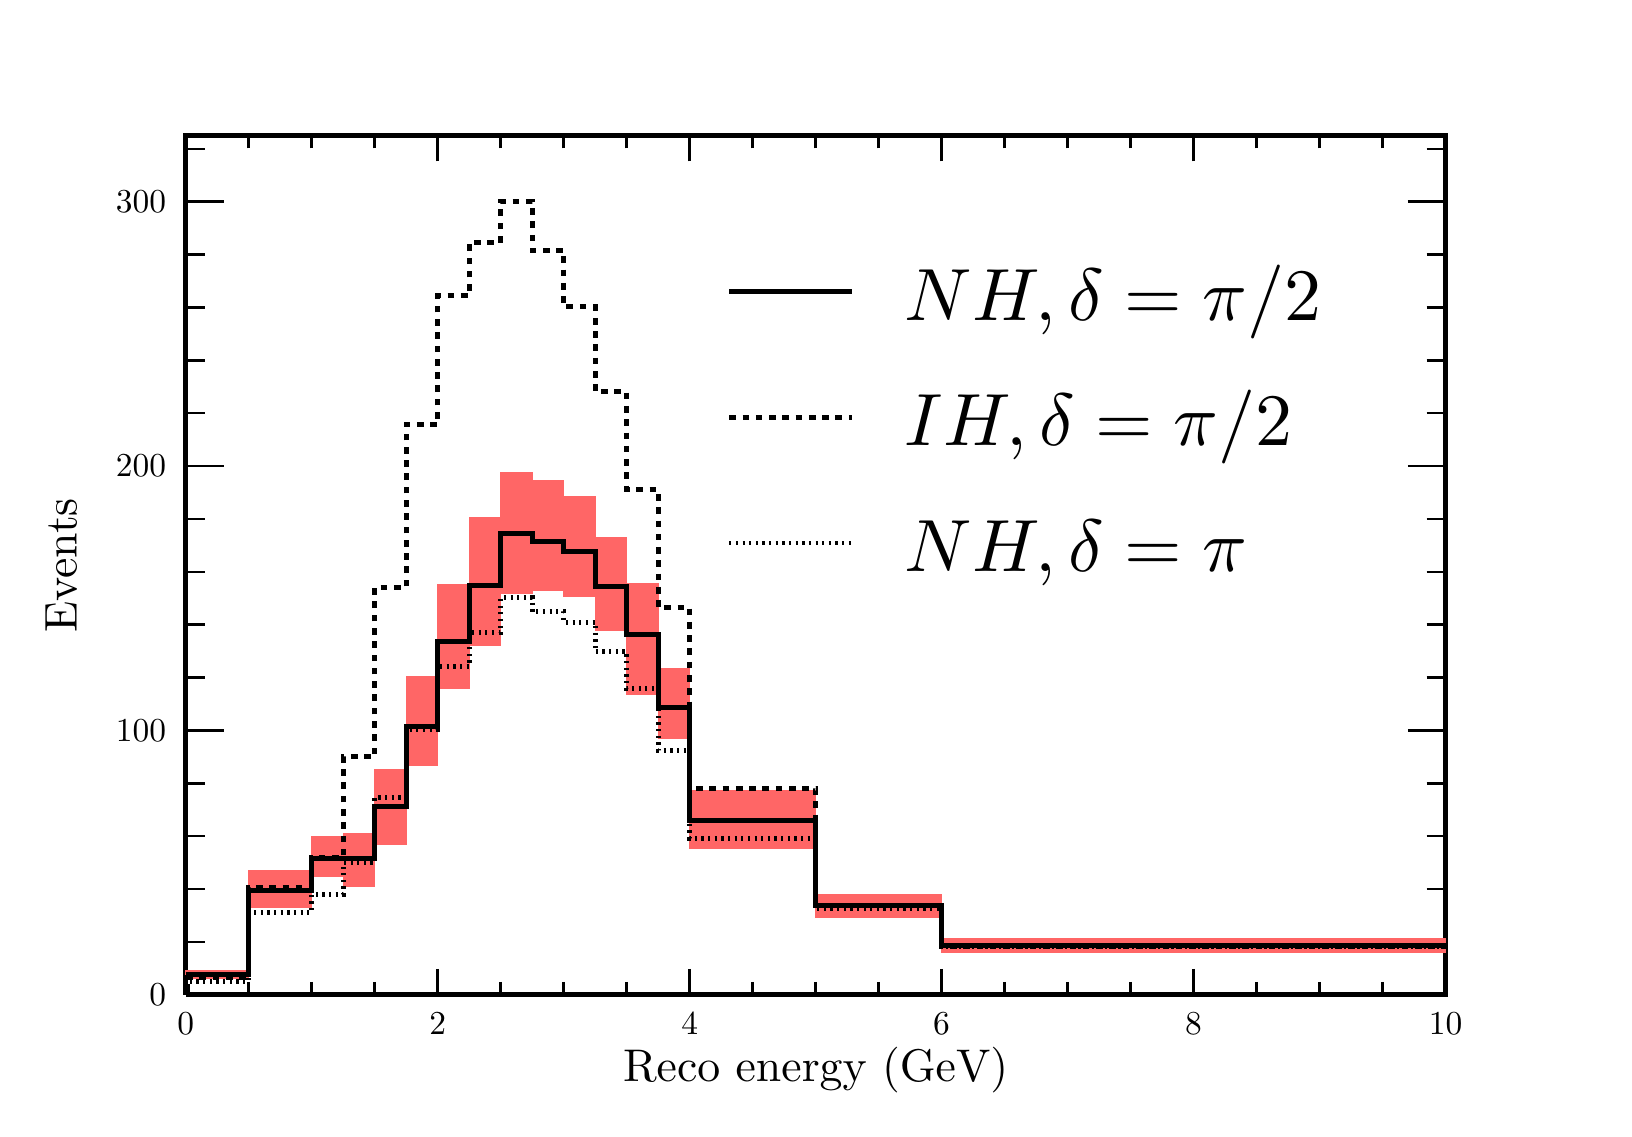
\begin{tikzpicture}
\pgfdeclareplotmark{cross} {
\pgfpathmoveto{\pgfpoint{-0.3\pgfplotmarksize}{\pgfplotmarksize}}
\pgfpathlineto{\pgfpoint{+0.3\pgfplotmarksize}{\pgfplotmarksize}}
\pgfpathlineto{\pgfpoint{+0.3\pgfplotmarksize}{0.3\pgfplotmarksize}}
\pgfpathlineto{\pgfpoint{+1\pgfplotmarksize}{0.3\pgfplotmarksize}}
\pgfpathlineto{\pgfpoint{+1\pgfplotmarksize}{-0.3\pgfplotmarksize}}
\pgfpathlineto{\pgfpoint{+0.3\pgfplotmarksize}{-0.3\pgfplotmarksize}}
\pgfpathlineto{\pgfpoint{+0.3\pgfplotmarksize}{-1.\pgfplotmarksize}}
\pgfpathlineto{\pgfpoint{-0.3\pgfplotmarksize}{-1.\pgfplotmarksize}}
\pgfpathlineto{\pgfpoint{-0.3\pgfplotmarksize}{-0.3\pgfplotmarksize}}
\pgfpathlineto{\pgfpoint{-1.\pgfplotmarksize}{-0.3\pgfplotmarksize}}
\pgfpathlineto{\pgfpoint{-1.\pgfplotmarksize}{0.3\pgfplotmarksize}}
\pgfpathlineto{\pgfpoint{-0.3\pgfplotmarksize}{0.3\pgfplotmarksize}}
\pgfpathclose
\pgfusepathqstroke
}
\pgfdeclareplotmark{cross*} {
\pgfpathmoveto{\pgfpoint{-0.3\pgfplotmarksize}{\pgfplotmarksize}}
\pgfpathlineto{\pgfpoint{+0.3\pgfplotmarksize}{\pgfplotmarksize}}
\pgfpathlineto{\pgfpoint{+0.3\pgfplotmarksize}{0.3\pgfplotmarksize}}
\pgfpathlineto{\pgfpoint{+1\pgfplotmarksize}{0.3\pgfplotmarksize}}
\pgfpathlineto{\pgfpoint{+1\pgfplotmarksize}{-0.3\pgfplotmarksize}}
\pgfpathlineto{\pgfpoint{+0.3\pgfplotmarksize}{-0.3\pgfplotmarksize}}
\pgfpathlineto{\pgfpoint{+0.3\pgfplotmarksize}{-1.\pgfplotmarksize}}
\pgfpathlineto{\pgfpoint{-0.3\pgfplotmarksize}{-1.\pgfplotmarksize}}
\pgfpathlineto{\pgfpoint{-0.3\pgfplotmarksize}{-0.3\pgfplotmarksize}}
\pgfpathlineto{\pgfpoint{-1.\pgfplotmarksize}{-0.3\pgfplotmarksize}}
\pgfpathlineto{\pgfpoint{-1.\pgfplotmarksize}{0.3\pgfplotmarksize}}
\pgfpathlineto{\pgfpoint{-0.3\pgfplotmarksize}{0.3\pgfplotmarksize}}
\pgfpathclose
\pgfusepathqfillstroke
}
\pgfdeclareplotmark{newstar} {
\pgfpathmoveto{\pgfqpoint{0pt}{\pgfplotmarksize}}
\pgfpathlineto{\pgfqpointpolar{44}{0.5\pgfplotmarksize}}
\pgfpathlineto{\pgfqpointpolar{18}{\pgfplotmarksize}}
\pgfpathlineto{\pgfqpointpolar{-20}{0.5\pgfplotmarksize}}
\pgfpathlineto{\pgfqpointpolar{-54}{\pgfplotmarksize}}
\pgfpathlineto{\pgfqpointpolar{-90}{0.5\pgfplotmarksize}}
\pgfpathlineto{\pgfqpointpolar{234}{\pgfplotmarksize}}
\pgfpathlineto{\pgfqpointpolar{198}{0.5\pgfplotmarksize}}
\pgfpathlineto{\pgfqpointpolar{162}{\pgfplotmarksize}}
\pgfpathlineto{\pgfqpointpolar{134}{0.5\pgfplotmarksize}}
\pgfpathclose
\pgfusepathqstroke
}
\pgfdeclareplotmark{newstar*} {
\pgfpathmoveto{\pgfqpoint{0pt}{\pgfplotmarksize}}
\pgfpathlineto{\pgfqpointpolar{44}{0.5\pgfplotmarksize}}
\pgfpathlineto{\pgfqpointpolar{18}{\pgfplotmarksize}}
\pgfpathlineto{\pgfqpointpolar{-20}{0.5\pgfplotmarksize}}
\pgfpathlineto{\pgfqpointpolar{-54}{\pgfplotmarksize}}
\pgfpathlineto{\pgfqpointpolar{-90}{0.5\pgfplotmarksize}}
\pgfpathlineto{\pgfqpointpolar{234}{\pgfplotmarksize}}
\pgfpathlineto{\pgfqpointpolar{198}{0.5\pgfplotmarksize}}
\pgfpathlineto{\pgfqpointpolar{162}{\pgfplotmarksize}}
\pgfpathlineto{\pgfqpointpolar{134}{0.5\pgfplotmarksize}}
\pgfpathclose
\pgfusepathqfillstroke
}
\definecolor{c}{rgb}{0.999,0.999,0.999};
\draw [color=c, fill=c] (0,0) rectangle (20,13.639);
\draw [color=c, fill=c] (2,1.3639) rectangle (18,12.2751);
\definecolor{c}{rgb}{0,0,0};
\draw [c,line width=1.8] (2,1.3639) -- (2,12.2751) -- (18,12.2751) -- (18,1.3639) -- (2,1.3639);
\definecolor{c}{rgb}{0.999,0.999,0.999};
\draw [color=c, fill=c] (2,1.3639) rectangle (18,12.2751);
\definecolor{c}{rgb}{0,0,0};
\draw [c,line width=1.8] (2,1.3639) -- (2,12.2751) -- (18,12.2751) -- (18,1.3639) -- (2,1.3639);
\draw [c,line width=1.8] (2,1.6177) -- (2.8,1.6177) -- (2.8,2.68844) -- (3.6,2.68844) -- (3.6,3.09122) -- (4,3.09122) -- (4,3.08849) -- (4.4,3.08849) -- (4.4,3.75008) -- (4.8,3.75008) -- (4.8,4.76675) -- (5.2,4.76675) -- (5.2,5.85521) --
 (5.6,5.85521) -- (5.6,6.56073) -- (6,6.56073) -- (6,7.21918) -- (6.4,7.21918) -- (6.4,7.12647) -- (6.8,7.12647) -- (6.8,6.99581) -- (7.2,6.99581) -- (7.2,6.54549) -- (7.6,6.54549) -- (7.6,5.94198) -- (8,5.94198) -- (8,5.00812) -- (8.4,5.00812) --
 (8.4,3.57712) -- (10,3.57712) -- (10,2.49612) -- (11.6,2.49612) -- (11.6,1.98899) -- (18,1.98899);
\draw [c,line width=0.9] (2,1.3639) -- (18,1.3639);
\draw [c,line width=0.9] (2,1.69123) -- (2,1.3639);
\draw [c,line width=0.9] (2.8,1.52756) -- (2.8,1.3639);
\draw [c,line width=0.9] (3.6,1.52756) -- (3.6,1.3639);
\draw [c,line width=0.9] (4.4,1.52756) -- (4.4,1.3639);
\draw [c,line width=0.9] (5.2,1.69123) -- (5.2,1.3639);
\draw [c,line width=0.9] (6,1.52756) -- (6,1.3639);
\draw [c,line width=0.9] (6.8,1.52756) -- (6.8,1.3639);
\draw [c,line width=0.9] (7.6,1.52756) -- (7.6,1.3639);
\draw [c,line width=0.9] (8.4,1.69123) -- (8.4,1.3639);
\draw [c,line width=0.9] (9.2,1.52756) -- (9.2,1.3639);
\draw [c,line width=0.9] (10,1.52756) -- (10,1.3639);
\draw [c,line width=0.9] (10.8,1.52756) -- (10.8,1.3639);
\draw [c,line width=0.9] (11.6,1.69123) -- (11.6,1.3639);
\draw [c,line width=0.9] (12.4,1.52756) -- (12.4,1.3639);
\draw [c,line width=0.9] (13.2,1.52756) -- (13.2,1.3639);
\draw [c,line width=0.9] (14,1.52756) -- (14,1.3639);
\draw [c,line width=0.9] (14.8,1.69123) -- (14.8,1.3639);
\draw [c,line width=0.9] (15.6,1.52756) -- (15.6,1.3639);
\draw [c,line width=0.9] (16.4,1.52756) -- (16.4,1.3639);
\draw [c,line width=0.9] (17.2,1.52756) -- (17.2,1.3639);
\draw [c,line width=0.9] (18,1.69123) -- (18,1.3639);
\draw [anchor=base] (2,0.859255) node[scale=1.20912, color=c, rotate=0]{0};
\draw [anchor=base] (5.2,0.859255) node[scale=1.20912, color=c, rotate=0]{2};
\draw [anchor=base] (8.4,0.859255) node[scale=1.20912, color=c, rotate=0]{4};
\draw [anchor=base] (11.6,0.859255) node[scale=1.20912, color=c, rotate=0]{6};
\draw [anchor=base] (14.8,0.859255) node[scale=1.20912, color=c, rotate=0]{8};
\draw [anchor=base] (18,0.859255) node[scale=1.20912, color=c, rotate=0]{10};
\draw (10,0.403714) node[scale=1.65459, color=c, rotate=0]{Reco energy (GeV)};
\draw [c,line width=0.9] (2,12.2751) -- (18,12.2751);
\draw [c,line width=0.9] (2,11.9477) -- (2,12.2751);
\draw [c,line width=0.9] (2.8,12.1114) -- (2.8,12.2751);
\draw [c,line width=0.9] (3.6,12.1114) -- (3.6,12.2751);
\draw [c,line width=0.9] (4.4,12.1114) -- (4.4,12.2751);
\draw [c,line width=0.9] (5.2,11.9477) -- (5.2,12.2751);
\draw [c,line width=0.9] (6,12.1114) -- (6,12.2751);
\draw [c,line width=0.9] (6.8,12.1114) -- (6.8,12.2751);
\draw [c,line width=0.9] (7.6,12.1114) -- (7.6,12.2751);
\draw [c,line width=0.9] (8.4,11.9477) -- (8.4,12.2751);
\draw [c,line width=0.9] (9.2,12.1114) -- (9.2,12.2751);
\draw [c,line width=0.9] (10,12.1114) -- (10,12.2751);
\draw [c,line width=0.9] (10.8,12.1114) -- (10.8,12.2751);
\draw [c,line width=0.9] (11.6,11.9477) -- (11.6,12.2751);
\draw [c,line width=0.9] (12.4,12.1114) -- (12.4,12.2751);
\draw [c,line width=0.9] (13.2,12.1114) -- (13.2,12.2751);
\draw [c,line width=0.9] (14,12.1114) -- (14,12.2751);
\draw [c,line width=0.9] (14.8,11.9477) -- (14.8,12.2751);
\draw [c,line width=0.9] (15.6,12.1114) -- (15.6,12.2751);
\draw [c,line width=0.9] (16.4,12.1114) -- (16.4,12.2751);
\draw [c,line width=0.9] (17.2,12.1114) -- (17.2,12.2751);
\draw [c,line width=0.9] (18,11.9477) -- (18,12.2751);
\draw [c,line width=0.9] (2,1.3639) -- (2,12.2751);
\draw [c,line width=0.9] (2.48,1.3639) -- (2,1.3639);
\draw [c,line width=0.9] (2.24,2.03535) -- (2,2.03535);
\draw [c,line width=0.9] (2.24,2.70681) -- (2,2.70681);
\draw [c,line width=0.9] (2.24,3.37827) -- (2,3.37827);
\draw [c,line width=0.9] (2.24,4.04972) -- (2,4.04972);
\draw [c,line width=0.9] (2.48,4.72118) -- (2,4.72118);
\draw [c,line width=0.9] (2.24,5.39264) -- (2,5.39264);
\draw [c,line width=0.9] (2.24,6.0641) -- (2,6.0641);
\draw [c,line width=0.9] (2.24,6.73555) -- (2,6.73555);
\draw [c,line width=0.9] (2.24,7.40701) -- (2,7.40701);
\draw [c,line width=0.9] (2.48,8.07847) -- (2,8.07847);
\draw [c,line width=0.9] (2.24,8.74992) -- (2,8.74992);
\draw [c,line width=0.9] (2.24,9.42138) -- (2,9.42138);
\draw [c,line width=0.9] (2.24,10.0928) -- (2,10.0928);
\draw [c,line width=0.9] (2.24,10.7643) -- (2,10.7643);
\draw [c,line width=0.9] (2.48,11.4358) -- (2,11.4358);
\draw [c,line width=0.9] (2.48,11.4358) -- (2,11.4358);
\draw [c,line width=0.9] (2.24,12.1072) -- (2,12.1072);
\draw [anchor= east] (1.9,1.3639) node[scale=1.20912, color=c, rotate=0]{0};
\draw [anchor= east] (1.9,4.72118) node[scale=1.20912, color=c, rotate=0]{100};
\draw [anchor= east] (1.9,8.07847) node[scale=1.20912, color=c, rotate=0]{200};
\draw [anchor= east] (1.9,11.4358) node[scale=1.20912, color=c, rotate=0]{300};
\draw (0.416,6.81948) node[scale=1.65459, color=c, rotate=90]{Events};
\draw [c,line width=0.9] (18,1.3639) -- (18,12.2751);
\draw [c,line width=0.9] (17.52,1.3639) -- (18,1.3639);
\draw [c,line width=0.9] (17.76,2.03535) -- (18,2.03535);
\draw [c,line width=0.9] (17.76,2.70681) -- (18,2.70681);
\draw [c,line width=0.9] (17.76,3.37827) -- (18,3.37827);
\draw [c,line width=0.9] (17.76,4.04972) -- (18,4.04972);
\draw [c,line width=0.9] (17.52,4.72118) -- (18,4.72118);
\draw [c,line width=0.9] (17.76,5.39264) -- (18,5.39264);
\draw [c,line width=0.9] (17.76,6.0641) -- (18,6.0641);
\draw [c,line width=0.9] (17.76,6.73555) -- (18,6.73555);
\draw [c,line width=0.9] (17.76,7.40701) -- (18,7.40701);
\draw [c,line width=0.9] (17.52,8.07847) -- (18,8.07847);
\draw [c,line width=0.9] (17.76,8.74992) -- (18,8.74992);
\draw [c,line width=0.9] (17.76,9.42138) -- (18,9.42138);
\draw [c,line width=0.9] (17.76,10.0928) -- (18,10.0928);
\draw [c,line width=0.9] (17.76,10.7643) -- (18,10.7643);
\draw [c,line width=0.9] (17.52,11.4358) -- (18,11.4358);
\draw [c,line width=0.9] (17.52,11.4358) -- (18,11.4358);
\draw [c,line width=0.9] (17.76,12.1072) -- (18,12.1072);
\definecolor{c}{rgb}{1,0.4,0.4};
\draw [color=c, fill=c] (2,1.56583) rectangle (2.8,1.67706);
\draw [color=c, fill=c] (2.8,2.47101) rectangle (3.6,2.93721);
\draw [color=c, fill=c] (3.6,2.86112) rectangle (4,3.3723);
\draw [color=c, fill=c] (4,2.74153) rectangle (4.4,3.40935);
\draw [color=c, fill=c] (4.4,3.27555) rectangle (4.8,4.21832);
\draw [color=c, fill=c] (4.8,4.27587) rectangle (5.2,5.40328);
\draw [color=c, fill=c] (5.2,5.25327) rectangle (5.6,6.57743);
\draw [color=c, fill=c] (5.6,5.80297) rectangle (6,7.42178);
\draw [color=c, fill=c] (6,6.46267) rectangle (6.4,7.99531);
\draw [color=c, fill=c] (6.4,6.4933) rectangle (6.8,7.90008);
\draw [color=c, fill=c] (6.8,6.42671) rectangle (7.2,7.69297);
\draw [color=c, fill=c] (7.2,5.98745) rectangle (7.6,7.16849);
\draw [color=c, fill=c] (7.6,5.17805) rectangle (8,6.58456);
\draw [color=c, fill=c] (8,4.61291) rectangle (8.4,5.51272);
\draw [color=c, fill=c] (8.4,3.2252) rectangle (10,3.9541);
\draw [color=c, fill=c] (10,2.3515) rectangle (11.6,2.64007);
\draw [color=c, fill=c] (11.6,1.89867) rectangle (18,2.08046);
\definecolor{c}{rgb}{0,0,0};
\draw [c,line width=1.8] (2,1.6177) -- (2.8,1.6177) -- (2.8,2.68844) -- (3.6,2.68844) -- (3.6,3.09122) -- (4,3.09122) -- (4,3.08849) -- (4.4,3.08849) -- (4.4,3.75008) -- (4.8,3.75008) -- (4.8,4.76675) -- (5.2,4.76675) -- (5.2,5.85521) --
 (5.6,5.85521) -- (5.6,6.56073) -- (6,6.56073) -- (6,7.21918) -- (6.4,7.21918) -- (6.4,7.12647) -- (6.8,7.12647) -- (6.8,6.99581) -- (7.2,6.99581) -- (7.2,6.54549) -- (7.6,6.54549) -- (7.6,5.94198) -- (8,5.94198) -- (8,5.00812) -- (8.4,5.00812) --
 (8.4,3.57712) -- (10,3.57712) -- (10,2.49612) -- (11.6,2.49612) -- (11.6,1.98899) -- (18,1.98899);
\draw [c,dash pattern=on 2.40pt off 2.40pt ,line width=1.8] (2.02865,1.39255) -- (2.02865,1.58348) -- (2.8,1.58348) -- (2.8,2.72171) -- (3.6,2.72171) -- (3.6,3.10463) -- (4,3.10463) -- (4,4.38373) -- (4.4,4.38373) -- (4.4,6.53775) -- (4.8,6.53775) --
 (4.8,8.6076) -- (5.2,8.6076) -- (5.2,10.2407) -- (5.6,10.2407) -- (5.6,10.9166) -- (6,10.9166) -- (6,11.4413) -- (6.4,11.4413) -- (6.4,10.8176) -- (6.8,10.8176) -- (6.8,10.1021) -- (7.2,10.1021) -- (7.2,9.02097) -- (7.6,9.02097) -- (7.6,7.78272) --
 (8,7.78272) -- (8,6.28234) -- (8.4,6.28234) -- (8.4,3.98728) -- (10,3.98728) -- (10,2.50318) -- (11.6,2.50318) -- (11.6,1.98241) -- (18,1.98241);
\draw [c,dash pattern=on 0.80pt off 1.60pt ,line width=1.8] (2.02865,1.39255) -- (2.02865,1.53772) -- (2.8,1.53772) -- (2.8,2.40784) -- (3.6,2.40784) -- (3.6,2.63669) -- (4,2.63669) -- (4,3.03935) -- (4.4,3.03935) -- (4.4,3.86671) -- (4.8,3.86671) --
 (4.8,4.73566) -- (5.2,4.73566) -- (5.2,5.52994) -- (5.6,5.52994) -- (5.6,5.9674) -- (6,5.9674) -- (6,6.40553) -- (6.4,6.40553) -- (6.4,6.22543) -- (6.8,6.22543) -- (6.8,6.09706) -- (7.2,6.09706) -- (7.2,5.71752) -- (7.6,5.71752) -- (7.6,5.24812) --
 (8,5.24812) -- (8,4.4707) -- (8.4,4.4707) -- (8.4,3.34666) -- (10,3.34666) -- (10,2.45385) -- (11.6,2.45385) -- (11.6,1.97765) -- (18,1.97765);
\definecolor{c}{rgb}{1,1,1};
\draw [color=c, fill=c] (8.56734,6.30372) rectangle (17.5072,11.0888);
\definecolor{c}{rgb}{0,0,0};
\draw [anchor=base west] (10.8023,9.93243) node[scale=2.6728, color=c, rotate=0]{$NH, \delta = \pi/2$};
\draw [c,line width=1.8] (8.90258,10.2913) -- (10.467,10.2913);
\draw [anchor=base west] (10.8023,8.33739) node[scale=2.6728, color=c, rotate=0]{$IH, \delta = \pi/2$};
\draw [c,dash pattern=on 2.40pt off 2.40pt ,line width=1.8] (8.90258,8.69627) -- (10.467,8.69627);
\draw [anchor=base west] (10.8023,6.74236) node[scale=2.6728, color=c, rotate=0]{$NH, \delta = \pi$};
\draw [c,dash pattern=on 0.80pt off 1.60pt ,line width=1.8] (8.90258,7.10124) -- (10.467,7.10124);
\end{tikzpicture}
